\documentclass[journal]{IEEEtran}
\usepackage[dvipdfmx]{graphicx}
\usepackage{ascmac}
\usepackage{docmute}
\usepackage{comment}
\usepackage{listings}
\usepackage{listings}
\lstset{
	%枠外での自動改行
 	breaklines = true,
 	%標準の書体
 	%basicstyle = {\small},
 	%枠 "t"は上に線を記載, "T"は上に二重線を記載
	%他オプション:leftline,topline,bottomline,lines,single,shadowbox
 	frame = TB,
 	%タブの大きさ
 	tabsize = 2,
 	%キャプションの場所("tb"ならば上下両方に記載)
 	%captionpos = t,
 	%行番号の位置
 	%numbers = left,
 	%自動改行後のインデント量(デフォルトでは20[pt])	
 	breakindent = 30pt,
	%左右の位置調整 	
 	xleftmargin=15pt,
 	xrightmargin=10pt,
	%プログラム言語(複数の言語に対応,C,C++も可)
 	%language = Python, 	
 	%背景色と透過度
 	%backgroundcolor={\color[gray]{.90}},
 	%コメントの書体
 	%commentstyle = {\itshape \color[cmyk]{1,0.4,1,0}},
 	%関数名等の色の設定
 	%classoffset = 0,
 	%キーワード(int, ifなど)の書体
 	%keywordstyle = {\bfseries \color[cmyk]{0,1,0,0}},
 	%表示する文字の書体
 	%stringstyle = {\ttfamily \color[rgb]{0,0,1}},
 	%frameまでの間隔(行番号とプログラムの間)
 	%framesep = 5pt,
 	%行番号の間隔
 	%stepnumber = 1,
	%行番号の書体
 	%numberstyle = \tiny,
}
\makeatletter
\def\lst@makecaption{%
  \def\@captype{table}%
  \@makecaption
}
\makeatother
\renewcommand{\lstlistingname}{Code}

% Some very useful LaTeX packages include:
% (uncomment the ones you want to load)


% *** MISC UTILITY PACKAGES ***
%
%\usepackage{ifpdf}
% Heiko Oberdiek's ifpdf.sty is very useful if you need conditional
% compilation based on whether the output is pdf or dvi.
% usage:
% \ifpdf
%   % pdf code
% \else
%   % dvi code
% \fi
% The latest version of ifpdf.sty can be obtained from:
% http://www.ctan.org/pkg/ifpdf
% Also, note that IEEEtran.cls V1.7 and later provides a builtin
% \ifCLASSINFOpdf conditional that works the same way.
% When switching from latex to pdflatex and vice-versa, the compiler may
% have to be run twice to clear warning/error messages.


% *** CITATION PACKAGES ***
%
\usepackage{cite}
% cite.sty was written by Donald Arseneau
% V1.6 and later of IEEEtran pre-defines the format of the cite.sty package
% \cite{} output to follow that of the IEEE. Loading the cite package will
% result in citation numbers being automatically sorted and properly
% "compressed/ranged". e.g., [1], [9], [2], [7], [5], [6] without using
% cite.sty will become [1], [2], [5]--[7], [9] using cite.sty. cite.sty's
% \cite will automatically add leading space, if needed. Use cite.sty's
% noadjust option (cite.sty V3.8 and later) if you want to turn this off
% such as if a citation ever needs to be enclosed in parenthesis.
% cite.sty is already installed on most LaTeX systems. Be sure and use
% version 5.0 (2009-03-20) and later if using hyperref.sty.
% The latest version can be obtained at:
% http://www.ctan.org/pkg/cite
% The documentation is contained in the cite.sty file itself.


% *** GRAPHICS RELATED PACKAGES ***
%
\ifCLASSINFOpdf
  % \usepackage[pdftex]{graphicx}
  % declare the path(s) where your graphic files are
  % \graphicspath{{../pdf/}{../jpeg/}}
  % and their extensions so you won't have to specify these with
  % every instance of \includegraphics
  % \DeclareGraphicsExtensions{.pdf,.jpeg,.png}
\else
  % or other class option (dvipsone, dvipdf, if not using dvips). graphicx
  % will default to the driver specified in the system graphics.cfg if no
  % driver is specified.
  % \usepackage[dvips]{graphicx}
  % declare the path(s) where your graphic files are
  % \graphicspath{{../eps/}}
  % and their extensions so you won't have to specify these with
  % every instance of \includegraphics
  % \DeclareGraphicsExtensions{.eps}
\fi
% graphicx was written by David Carlisle and Sebastian Rahtz. It is
% required if you want graphics, photos, etc. graphicx.sty is already
% installed on most LaTeX systems. The latest version and documentation
% can be obtained at: 
% http://www.ctan.org/pkg/graphicx
% Another good source of documentation is "Using Imported Graphics in
% LaTeX2e" by Keith Reckdahl which can be found at:
% http://www.ctan.org/pkg/epslatex
%
% latex, and pdflatex in dvi mode, support graphics in encapsulated
% postscript (.eps) format. pdflatex in pdf mode supports graphics
% in .pdf, .jpeg, .png and .mps (metapost) formats. Users should ensure
% that all non-photo figures use a vector format (.eps, .pdf, .mps) and
% not a bitmapped formats (.jpeg, .png). The IEEE frowns on bitmapped formats
% which can result in "jaggedy"/blurry rendering of lines and letters as
% well as large increases in file sizes.
%
% You can find documentation about the pdfTeX application at:
% http://www.tug.org/applications/pdftex


% *** MATH PACKAGES ***
%
%\usepackage{amsmath}
% A popular package from the American Mathematical Society that provides
% many useful and powerful commands for dealing with mathematics.
%
% Note that the amsmath package sets \interdisplaylinepenalty to 10000
% thus preventing page breaks from occurring within multiline equations. Use:
%\interdisplaylinepenalty=2500
% after loading amsmath to restore such page breaks as IEEEtran.cls normally
% does. amsmath.sty is already installed on most LaTeX systems. The latest
% version and documentation can be obtained at:
% http://www.ctan.org/pkg/amsmath


% *** SPECIALIZED LIST PACKAGES ***
%
%\usepackage{algorithmic}
% algorithmic.sty was written by Peter Williams and Rogerio Brito.
% This package provides an algorithmic environment fo describing algorithms.
% You can use the algorithmic environment in-text or within a figure
% environment to provide for a floating algorithm. Do NOT use the algorithm
% floating environment provided by algorithm.sty (by the same authors) or
% algorithm2e.sty (by Christophe Fiorio) as the IEEE does not use dedicated
% algorithm float types and packages that provide these will not provide
% correct IEEE style captions. The latest version and documentation of
% algorithmic.sty can be obtained at:
% http://www.ctan.org/pkg/algorithms
% Also of interest may be the (relatively newer and more customizable)
% algorithmicx.sty package by Szasz Janos:
% http://www.ctan.org/pkg/algorithmicx


% *** ALIGNMENT PACKAGES ***
%
%\usepackage{array}
% Frank Mittelbach's and David Carlisle's array.sty patches and improves
% the standard LaTeX2e array and tabular environments to provide better
% appearance and additional user controls. As the default LaTeX2e table
% generation code is lacking to the point of almost being broken with
% respect to the quality of the end results, all users are strongly
% advised to use an enhanced (at the very least that provided by array.sty)
% set of table tools. array.sty is already installed on most systems. The
% latest version and documentation can be obtained at:
% http://www.ctan.org/pkg/array


% IEEEtran contains the IEEEeqnarray family of commands that can be used to
% generate multiline equations as well as matrices, tables, etc., of high
% quality.


% *** SUBFIGURE PACKAGES ***
%\ifCLASSOPTIONcompsoc
%  \usepackage[caption=false,font=normalsize,labelfont=sf,textfont=sf]{subfig}
%\else
%  \usepackage[caption=false,font=footnotesize]{subfig}
%\fi
% subfig.sty, written by Steven Douglas Cochran, is the modern replacement
% for subfigure.sty, the latter of which is no longer maintained and is
% incompatible with some LaTeX packages including fixltx2e. However,
% subfig.sty requires and automatically loads Axel Sommerfeldt's caption.sty
% which will override IEEEtran.cls' handling of captions and this will result
% in non-IEEE style figure/table captions. To prevent this problem, be sure
% and invoke subfig.sty's "caption=false" package option (available since
% subfig.sty version 1.3, 2005/06/28) as this is will preserve IEEEtran.cls
% handling of captions.
% Note that the Computer Society format requires a larger sans serif font
% than the serif footnote size font used in traditional IEEE formatting
% and thus the need to invoke different subfig.sty package options depending
% on whether compsoc mode has been enabled.
%
% The latest version and documentation of subfig.sty can be obtained at:
% http://www.ctan.org/pkg/subfig


% *** FLOAT PACKAGES ***
%
%\usepackage{fixltx2e}
% fixltx2e, the successor to the earlier fix2col.sty, was written by
% Frank Mittelbach and David Carlisle. This package corrects a few problems
% in the LaTeX2e kernel, the most notable of which is that in current
% LaTeX2e releases, the ordering of single and double column floats is not
% guaranteed to be preserved. Thus, an unpatched LaTeX2e can allow a
% single column figure to be placed prior to an earlier double column
% figure.
% Be aware that LaTeX2e kernels dated 2015 and later have fixltx2e.sty's
% corrections already built into the system in which case a warning will
% be issued if an attempt is made to load fixltx2e.sty as it is no longer
% needed.
% The latest version and documentation can be found at:
% http://www.ctan.org/pkg/fixltx2e


%\usepackage{stfloats}
% stfloats.sty was written by Sigitas Tolusis. This package gives LaTeX2e
% the ability to do double column floats at the bottom of the page as well
% as the top. (e.g., "\begin{figure*}[!b]" is not normally possible in
% LaTeX2e). It also provides a command:
%\fnbelowfloat
% to enable the placement of footnotes below bottom floats (the standard
% LaTeX2e kernel puts them above bottom floats). This is an invasive package
% which rewrites many portions of the LaTeX2e float routines. It may not work
% with other packages that modify the LaTeX2e float routines. The latest
% version and documentation can be obtained at:
% http://www.ctan.org/pkg/stfloats
% Do not use the stfloats baselinefloat ability as the IEEE does not allow
% \baselineskip to stretch. Authors submitting work to the IEEE should note
% that the IEEE rarely uses double column equations and that authors should try
% to avoid such use. Do not be tempted to use the cuted.sty or midfloat.sty
% packages (also by Sigitas Tolusis) as the IEEE does not format its papers in
% such ways.
% Do not attempt to use stfloats with fixltx2e as they are incompatible.
% Instead, use Morten Hogholm'a dblfloatfix which combines the features
% of both fixltx2e and stfloats:
%
% \usepackage{dblfloatfix}
% The latest version can be found at:
% http://www.ctan.org/pkg/dblfloatfix


%\ifCLASSOPTIONcaptionsoff
%  \usepackage[nomarkers]{endfloat}
% \let\MYoriglatexcaption\caption
% \renewcommand{\caption}[2][\relax]{\MYoriglatexcaption[#2]{#2}}
%\fi
% endfloat.sty was written by James Darrell McCauley, Jeff Goldberg and 
% Axel Sommerfeldt. This package may be useful when used in conjunction with 
% IEEEtran.cls'  captionsoff option. Some IEEE journals/societies require that
% submissions have lists of figures/tables at the end of the paper and that
% figures/tables without any captions are placed on a page by themselves at
% the end of the document. If needed, the draftcls IEEEtran class option or
% \CLASSINPUTbaselinestretch interface can be used to increase the line
% spacing as well. Be sure and use the nomarkers option of endfloat to
% prevent endfloat from "marking" where the figures would have been placed
% in the text. The two hack lines of code above are a slight modification of
% that suggested by in the endfloat docs (section 8.4.1) to ensure that
% the full captions always appear in the list of figures/tables - even if
% the user used the short optional argument of \caption[]{}.
% IEEE papers do not typically make use of \caption[]'s optional argument,
% so this should not be an issue. A similar trick can be used to disable
% captions of packages such as subfig.sty that lack options to turn off
% the subcaptions:
% For subfig.sty:
% \let\MYorigsubfloat\subfloat
% \renewcommand{\subfloat}[2][\relax]{\MYorigsubfloat[]{#2}}
% However, the above trick will not work if both optional arguments of
% the \subfloat command are used. Furthermore, there needs to be a
% description of each subfigure *somewhere* and endfloat does not add
% subfigure captions to its list of figures. Thus, the best approach is to
% avoid the use of subfigure captions (many IEEE journals avoid them anyway)
% and instead reference/explain all the subfigures within the main caption.
% The latest version of endfloat.sty and its documentation can obtained at:
% http://www.ctan.org/pkg/endfloat
%
% The IEEEtran \ifCLASSOPTIONcaptionsoff conditional can also be used
% later in the document, say, to conditionally put the References on a 
% page by themselves.


% *** PDF, URL AND HYPERLINK PACKAGES ***
%
%\usepackage{url}
% url.sty was written by Donald Arseneau. It provides better support for
% handling and breaking URLs. url.sty is already installed on most LaTeX
% systems. The latest version and documentation can be obtained at:
% http://www.ctan.org/pkg/url
% Basically, \url{my_url_here}.

\begin{document}

\section{事例研究}
本章では、複数の具体的な事例を取り上げ、提案モデルの表現能力の向上を確認する。

\subsection{キャッシュの基本動作}
本節では、提案モデルでキャッシュの動作の表現の可能性を確認する。
提案モデルにおいて、キャッシュは格納、再利用、検証の三つの動作を行うため、それぞれについてAlloy Analyzerの実行結果を確認する。

\subsubsection{レスポンスの格納}
レスポンスの格納動作を確認するため、実行結果からレスポンスの格納を含む結果を抽出する。
ここでは簡単のため、最も単純な二者間における通信で生じるレスポンスの格納を対象とし、Code\ref{code:test_store}を用いて出力を得る。
Code\ref{code:test_store}はクライアントとサーバの二者間における一組のリクエストとレスポンスの通信において、格納レスポンス集合に要素が存在するキャッシュの状態が存在する結果を出力するものである。

\begin{lstlisting}[caption=レスポンスの格納, label=code:test_store]
run test_store{
	#HTTPClient = 1
	#HTTPServer = 1
	#HTTPRequest = 1
	#HTTPResponse = 1
	some CacheState.dif.store
} for 2
\end{lstlisting}

得られる出力結果を整理し、図\ref{fig:TestStore}に示す。
図\ref{fig:TestStore}には、PrivateCache0を持つBrowser0とServer0間の、Request0とResponse0のトランザクションにおけるキャッシュの状態変化が示されている。
最初のRequest0時にはキャッシュの状態はCacheState0で示されており、CacheState0の変化要素を表すCacheDifItem0のstoreは空集合である。
しかし、Response0時には状態はCacheState1に変化しており、対応するCacheDifItem1がResponse0にstoreを指している。
以上より、図\ref{fig:TestStore}はあるトランザクションにおいて、レスポンスがブラウザキャッシュに格納されている状態を表しており、レスポンスの格納が表現可能であることが確認できる。

%\begin{figure}[htb]
%\centering
%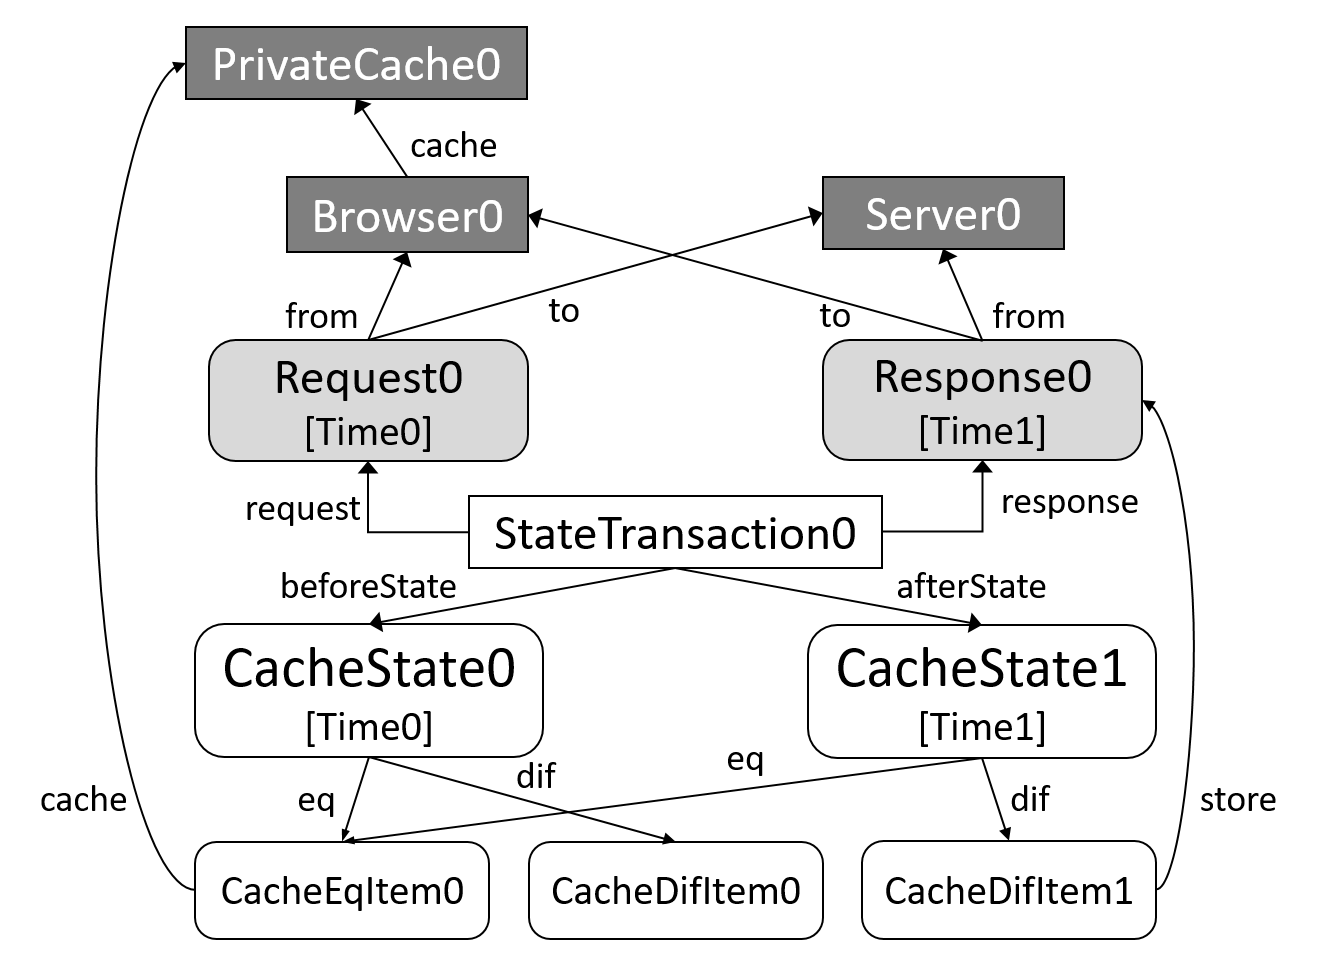
\includegraphics[width=450pt]{./fig/TestStore.eps}
%\caption{レスポンスを格納する状態の一例}
%\label{fig:TestStore}
%\end{figure}

\subsubsection{格納レスポンスの再利用}
レスポンスの再利用動作を確認するため、実行結果からレスポンスの再利用を含む結果を抽出する。
ここでは簡単のため、最も単純な二者間における通信で生じるレスポンスの再利用を対象とし、Code\ref{code:test_reuse}を用いて出力を得る。
Code\ref{code:test_reuse}はクライアントとサーバの二者間における二組の通信において、一度レスポンスの再利用が発生している結果を出力するものである。

\begin{lstlisting}[caption=格納レスポンスの再利用, label=code:test_reuse]
run test_reuse{
	#HTTPClient = 1
	#HTTPServer = 1
	#Cache = 1

	#HTTPRequest = 2
	#HTTPResponse = 1
	#CacheReuse = 1
} for 4
\end{lstlisting}

得られる出力結果をスペースの都合上、一部簡略化し図\ref{fig:TestReuse}に示す。
図\ref{fig:TestReuse}はあるキャッシュを持つブラウザとサーバ間で、同様のURIに対してリクエストが二回送信された状態を表している。
ここで、StateTransaction0では図\ref{fig:TestStore}と同様、ブラウザキャッシュにResponse0を格納している。
StateTransaction1では、この格納レスポンスを再利用するイベントCacheReuse0が発生している。
以上より、図\ref{fig:TestReuse}に示す出力結果から、再利用を伴う動作が表現可能であることが確認できる。

%\begin{figure}[htb]
%\centering
%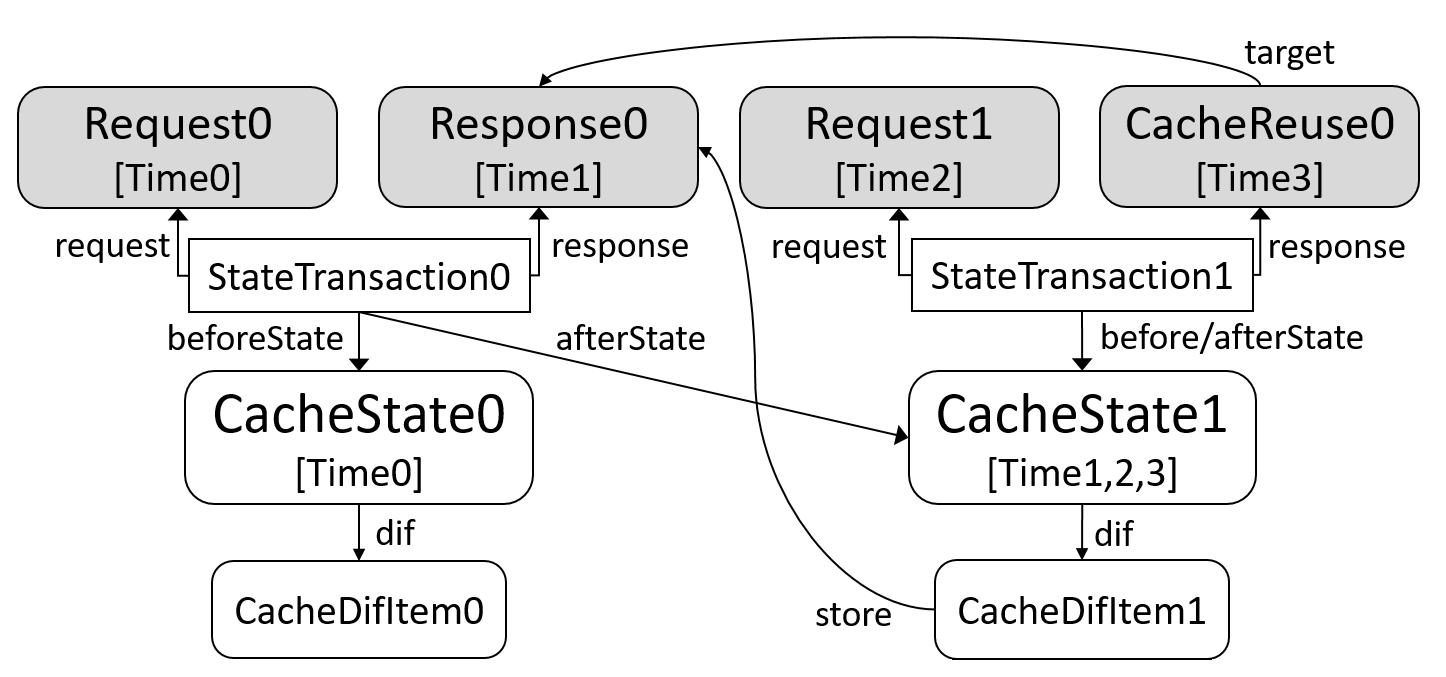
\includegraphics[width=450pt]{./fig/TestReuse.eps}
%\caption{格納レスポンスを再利用する状態の一例}
%\label{fig:TestReuse}
%\end{figure}

\subsubsection{格納レスポンスの検証}
レスポンスの検証動作を確認するため、実行結果からレスポンスの検証を含む結果を抽出する。
ここでは簡単のため、最も単純な二者間における通信で生じるレスポンスの検証を対象とし、Code\ref{code:test_verification}を用いて出力を得る。
Code\ref{code:test_verification}はクライアントとサーバの二者間における三組の通信のうち、検証が行われた通信が存在する結果を出力する。
ここでの検証の有無の判定は、\ref{sec:CacheVerification}節で述べた述語(Code\ref{code:checkVerification}参照)を利用している。

\begin{lstlisting}[caption=格納レスポンスの検証, label=code:test_verification]
run test_verification{
	#HTTPClient = 1
	#HTTPServer = 1
	#HTTPIntermediary = 0
	#Cache = 1
	#PrivateCache = 1

	some str:StateTransaction | checkVerification[str]
} for 6
\end{lstlisting}

得られる出力結果をスペースの都合上、一部簡略化し図\ref{fig:TestVerification}に示す。
図\ref{fig:TestVerification}はあるキャッシュを持つブラウザとサーバ間での三つの通信(StateTransaction0,1,2)が存在している状態を表しており、このうちStateTransaction2が検証を行っている通信である。
まず、StateTransaction0では図\ref{fig:TestStore}と同様、ブラウザキャッシュにResponse0を格納している。
次に、Request2に対してブラウザキャッシュ内に格納されているResponse0を再利用するため、StateTransaction2で検証動作を行っている。
ここで、格納レスポンスのResponse0にはEtagHeaderが含まれているため、検証に用いる条件付きリクエストであるRequest1にはIfNoneMatchHeaderが含まれている。
また、検証結果となるResponse1は再利用可能であることを示す304の状態コードとなっているため、Response0はそのまま再利用可能であることが示されている。
以上の流れからStateTransaction1ではResponse0をそのまま再利用しており、検証動作が正常に完了したことを示している。
よって、検証動作を表現可能であることが確認できる。

%\begin{figure}[htb]
%\centering
%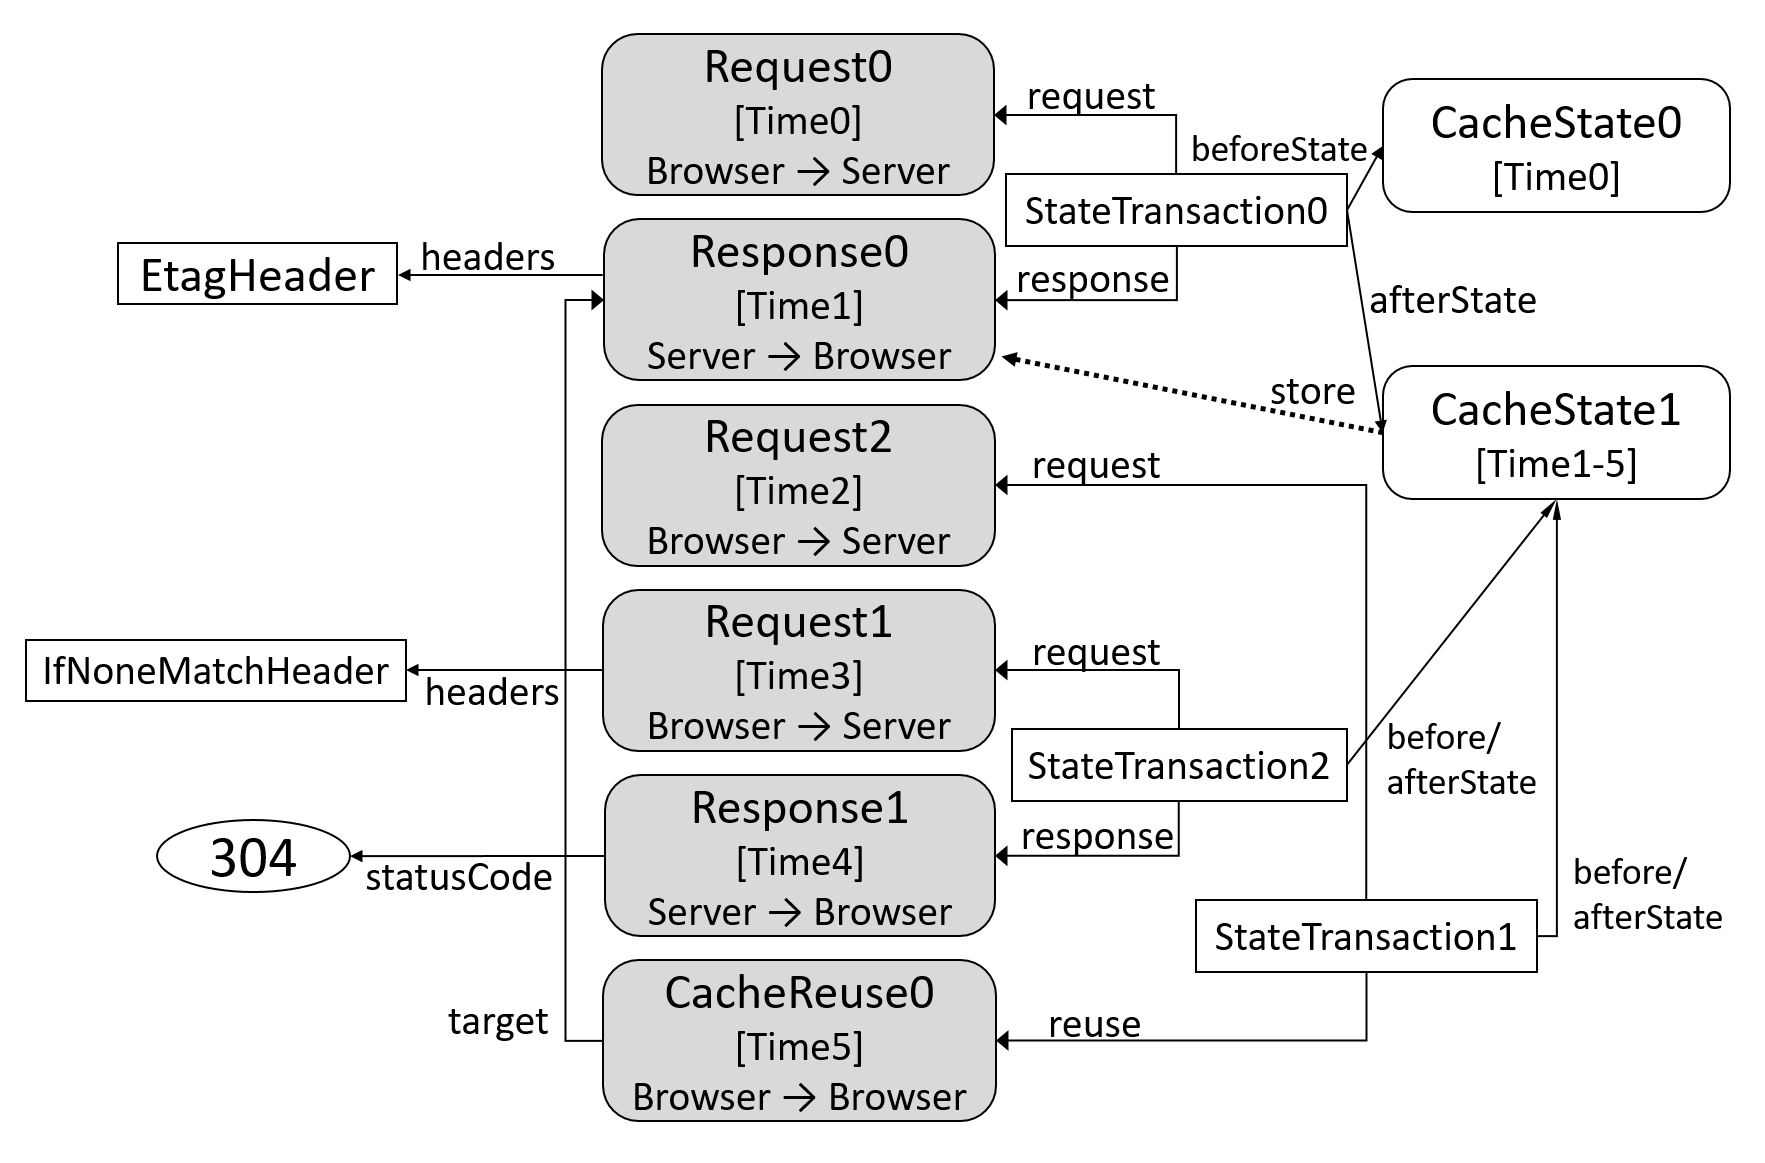
\includegraphics[width=450pt]{./fig/TestVerification.eps}
%\caption{格納レスポンスの検証が含まれる状態の一例}
%\label{fig:TestVerification}
%\end{figure}

\subsection{中継者の基本動作}
中継者の動作を確認するため、実行結果から中継者の動作を伴う動作を含む結果を抽出する。
ここでは簡単のため、最も単純なクライアント、中継者、サーバが各一つずつ存在する経路において、中継者を経由する通信を対象としCode\ref{code:test_intermediary}を用いて出力を得る。

\begin{lstlisting}[caption=中継者の動作, label=code:test_intermediary]
run test_intermediary{
	#HTTPRequest = 2
	#HTTPResponse = 2

	#HTTPClient = 1
	#HTTPServer = 1
	#HTTPIntermediary = 1

	all i:HTTPIntermediary | i in Alice.servers

	one req:HTTPRequest | req.to in HTTPIntermediary
	one req:HTTPRequest | req.to in HTTPServer
} for 4
\end{lstlisting}

得られる出力結果をスペースの都合上、一部簡略化し図\ref{fig:TestIntermediary}に示す。
図\ref{fig:TestIntermediary}で、HTTPTransaction0はブラウザと中継者間の通信、HTTPTransaction1は中継者とサーバ間の通信を表す。
中継者は自身に届けられたリクエストやレスポンスを回送する役割を持ち、このHTTPTransaction1がHTTPTransaction0を改装していることを表している。
以上より、中継者の動作が表現可能であることが確認できる。

%\begin{figure}[htb]
%\centering
%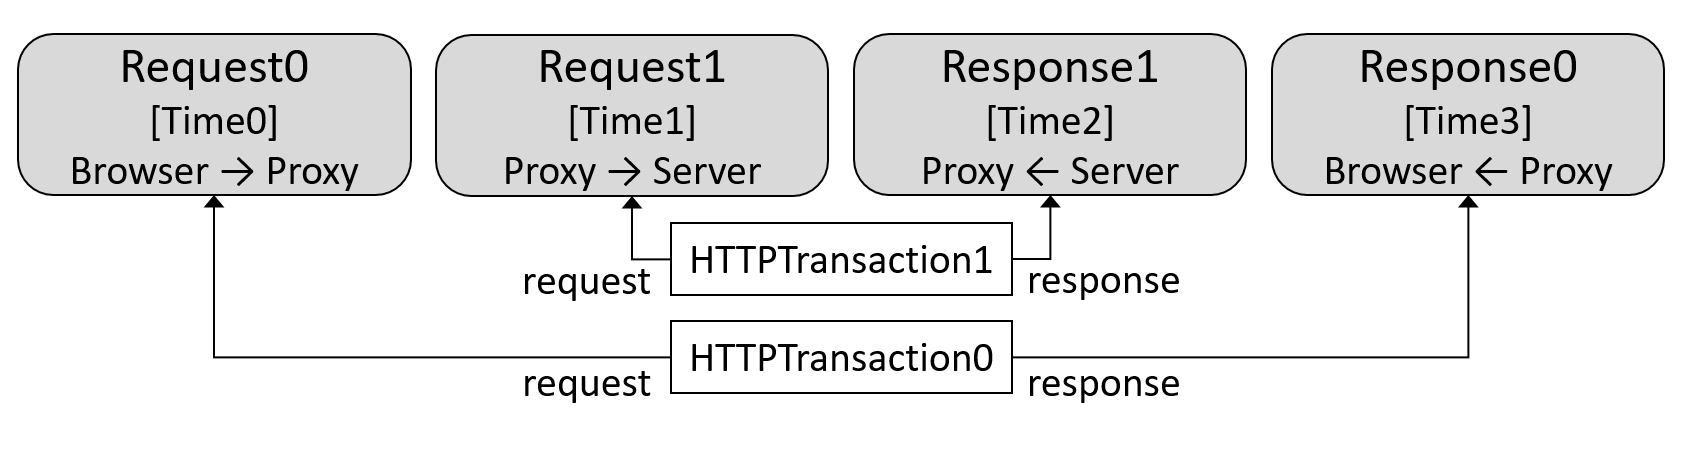
\includegraphics[width=450pt]{./fig/TestIntermediary.eps}
%\caption{中継者の動作を含む状態の一例}
%\label{fig:TestIntermediary}
%\end{figure}

\subsection{Same-origin Browser Cache Poisoning Attack}
\label{sec:same-origin-bcp}
本節では、提案モデルでSame-origin Browser Cache Poisoning Attack\cite{bcpattack}(以下、Same-origin BCP攻撃とする)が表現可能であるかを確認する。

Same-origin BCP攻撃は、攻撃者の持つ中継者が攻撃対象であるブラウザとサーバの経路上に入り込む「中間者攻撃」の一種である。
本攻撃の目的は対象のブラウザ、攻撃者の任意の動作を実行させることを目的とする。
また、本攻撃の特徴は、攻撃者による通信経路の割り込みが一度であるにも関わらず、そのレスポンスを再利用するたびにブラウザが悪影響を受けるという影響の持続性にある。

攻撃全体のフローを図\ref{fig:SameBCP_flow}に示す。
本攻撃による攻撃者のふるまいは、通信経路上において本来ブラウザが受け取るはずのレスポンスの内容に改ざん(図\ref{fig:SameBCP_flow}内の「4.改ざんレスポンス」)を行い、ブラウザが保有するキャッシュに改ざんレスポンスを格納させることである。
この際の攻撃者による改ざん内容は以下の二点である。
\begin{itemize}
\item レスポンスのヘッダをブラウザキャッシュによるレスポンスの格納や再利用を誘発するよう改ざんする。例えば、有効期限の延長や、検証動作なしの再利用の許可が挙げられる
\item レスポンスのボディに攻撃者に実行させたい任意の動作を記述する
\end{itemize}
また、ブラウザに悪影響が及ぶのは「5.改ざんレスポンスをキャッシュに格納」時と「6.同じファイルの利用時に改ざんレスポンスを再利用」時である。
また、6は改ざんレスポンスがキャッシュ内に格納されている間、何度も繰り返される可能性がある。

%\begin{figure}[htb]
%\centering
%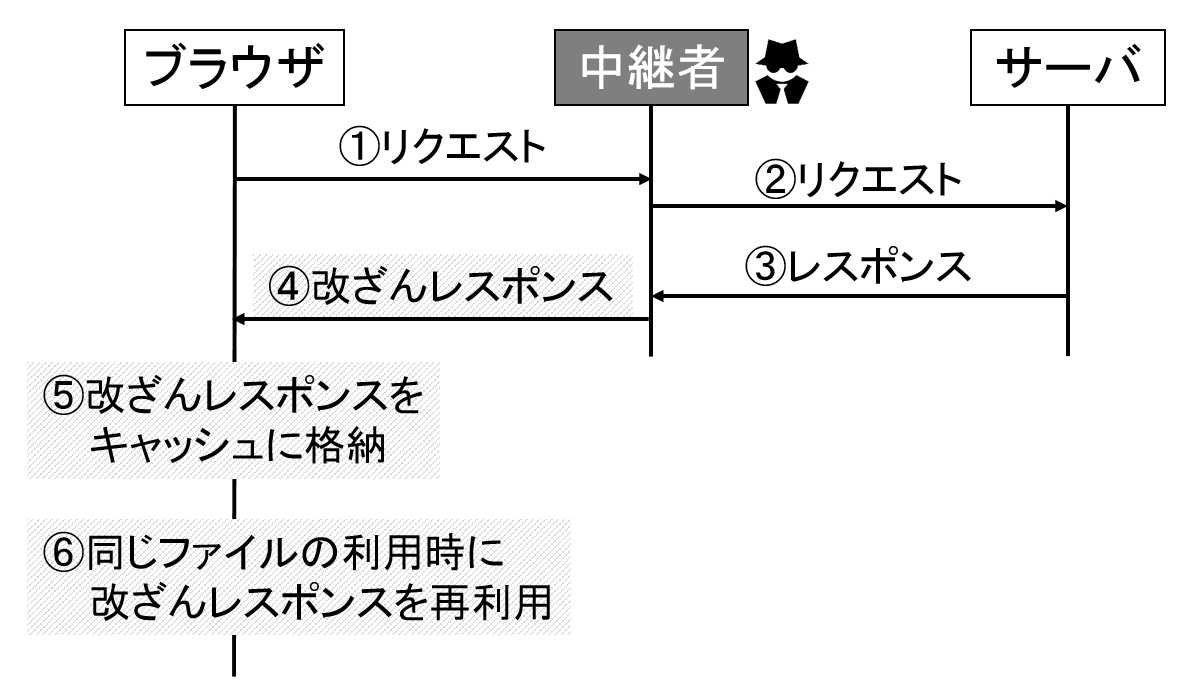
\includegraphics[width=400pt]{./fig/SameBCP_flow.eps}
%\caption{Same-origin Browser Cache Poisoning Attackの攻撃フロー}
%\label{fig:SameBCP_flow}
%\end{figure}

提案モデルによるSame-origin BCP攻撃の表現を確認するため、実行結果から図\ref{fig:SameBCP_flow}のフローを含む結果を抽出する。
抽出にはCode\ref{code:Same_origin_BCP}を用いる。
実行結果として、図\ref{fig:SameBCP_flow}に従ったフローと、攻撃者によるヘッダとボディの改ざんを含む状態が得られた。
このことから、提案モデルがSame-origin BCP攻撃を表現できることを確認した。

\begin{lstlisting}[caption=Same-origin BCP攻撃の表現, label=code:Same_origin_BCP]
run Same_origin_BCP{
	#HTTPClient = 1
	#HTTPServer = 1
	#HTTPIntermediary = 1
	#PrivateCache = 1
	#PublicCache = 0

	#HTTPRequest = 3
	#HTTPResponse = 2
	#CacheReuse = 1

	#Principal = 3
	#Alice = 2

	some tr,tr',tr'':HTTPTransaction | {
		tr'.request.current in tr.request.current.*next
		tr.response.current in tr'.response.current.*next
		tr''.request.current in tr.response.current.*next
		some tr''.re_res

		tr.request.from in HTTPClient
		tr.request.to in HTTPIntermediary

		tr'.request.from in HTTPIntermediary
		tr'.request.to in HTTPServer

		tr''.request.from in HTTPClient

		tr.response.body != tr'.response.body
	}

	some c:HTTPClient | c in Alice.httpClients
	some s:HTTPServer | s in Alice.servers
	no i:HTTPIntermediary | i in Alice.servers
} for 6
\end{lstlisting}

\subsection{Cross-site Request Forgery Attack}
本節では、提案モデルでCross-site Request Forgery Attack\cite{cookie-model}(以下、CSRF攻撃とする)が表現可能であるかを確認する。

CSRF攻撃は攻撃対象となるサーバと攻撃者が保有するサーバ、そして一般的なブラウザの三者間で実現される攻撃である。
本攻撃の目標は、攻撃対象であるサーバに対して、攻撃者が許されていない動作を実行させることである。

攻撃全体のフローを図\ref{fig:CSRF_flow}に示す。
本攻撃における攻撃者のふるまいは、自身が保有するサーバにアクセスしてきたブラウザが攻撃対象であるサーバへの「3.リクエスト」を送信を誘発するように「2.レスポンス」を返すことである。
また、この攻撃者からのレスポンスの内容によって、ブラウザから送信されるリクエストの内容も操作される。

%\begin{figure}[htb]
%\centering
%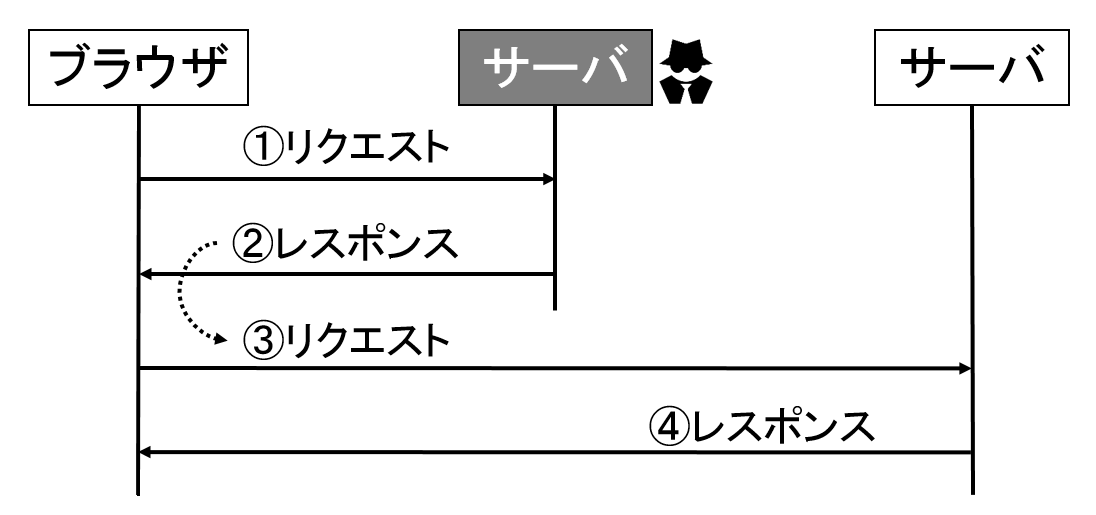
\includegraphics[width=400pt]{./fig/CSRF_flow.eps}
%\caption{Cross-site Request Forgery Attackの攻撃フロー}
%\label{fig:CSRF_flow}
%\end{figure}

提案モデルによるCSRF攻撃の表現を確認するため、実行結果から図\ref{fig:CSRF_flow}のフローを含む結果を抽出する。
抽出にはCode\ref{code:CSRF}を用い、その実行結果として図\ref{fig:CSRF_flow}に示す攻撃フローを含む結果が出力された。
スペースの都合上、これを一部簡略化し図\ref{fig:CSRF_alloy}に示す。
図\ref{fig:CSRF_alloy}において、Server0が攻撃者のサーバ、Server1が攻撃対象のサーバを表している。
また、HTTPTransaction0はBrowserがServer0にアクセスした通信を、HTTPTransaction1はそれに誘発されたBrowserとServer1の通信を表している。
HTTPTransaction1はHTTPTransaction0にcauseの関係を持ち、これがHTTPTransaction0に誘発されていることを示している。
以上のことから、CSRF攻撃を含む出力結果が得られているため、提案モデルがCSRF攻撃を表現できることを確認した。

\begin{lstlisting}[caption=CSRF攻撃の表現, label=code:CSRF]
run CSRF{
	#HTTPRequest = 2
	#HTTPResponse = 2

	#HTTPClient = 1
	#HTTPServer = 2
	#HTTPIntermediary = 0

	#Principal = 3
	#Alice = 2

	all p:Principal |
		one c:HTTPConformist |
			c in p.(servers + httpClients)
	all b:Browser | b in Alice.httpClients

	one tr1,tr2:HTTPTransaction|{
		tr2.request.current in tr1.response.current.*next

		tr1.request.to !in Alice.servers
		tr2.request.to in Alice.servers

		tr2.cause = tr1

		tr1.request.uri != tr2.request.uri
	}
} for 4
\end{lstlisting}

%\begin{figure}[htb]
%\centering
%\includegraphics[width=450pt]{./fig/CSRF_alloy.eps}
%\caption{CSRF攻撃のフローを含む状態の一例}
%\label{fig:CSRF_alloy}
%\end{figure}

\subsection{Cross-origin Browser Cache Poisoning Attack}
本節では、提案モデルでCross-origin Browser Cache Poisoning Attack\cite{bcpattack}(以下、Cross-origin BCP攻撃とする)が表現可能であるかを確認する。

Cross-origin BCP攻撃は、\ref{sec:same-origin-bcp}節で述べたSame-origin BCP攻撃と同様に「中間者攻撃」の一種である。
本攻撃法はSame-origin BCP攻撃に比べ、改ざんレスポンスの再利用の頻度を高めることができる。
これは、Cross-origin BCP攻撃では任意のファイルのレスポンスに改ざんを行うことができることに起因する。
これにより、一つのサイトだけでなく多くのサイトに共通して利用されるようなファイル(cssやjsファイルなど)を改ざんの対象とすることができる。
これに対して、\ref{sec:same-origin-bcp}節で記述のSame-origin BCP攻撃は、攻撃者がファイルを指定することはできず、通信に介入した際に偶然行われていた通信のみを改ざん可能な対象とする。

Cross-origin BCP攻撃は図\ref{fig:CrossBCP_flow}に示す攻撃フローで実現される。
ここで、図\ref{fig:CrossBCP_flow}内での「5.リクエスト」以降は、Same-origin BCP攻撃と同一のフローである。
また、それ以前のフローについては、CSRFのフローと役割が類似している。
まず最初に、攻撃者は「1.リクエスト」の通信に介入し、レスポンスの改ざんを行う。
ここにおける改ざんは、実際に改ざんを試みるファイルに対しての「5.リクエスト」の誘発を目的とする。
例えば、「A.css」という多くのページで共通して使用されるファイルが存在する場合、「3.レスポンス」の内容にA.cssを利用するよう追記することで、A.cssに対する「5.リクエスト」を誘発することができる。
したがって、図\ref{fig:CrossBCP_flow}のフローによって、攻撃者が指定する任意のファイルの改ざんを行い、そのレスポンスをブラウザキャッシュに格納させることができる。
また、このフローの成功後はサーバ1,2に無関係な通信であったとしても、改ざんレスポンスに記述されているファイルを利用する際には再利用が発生し、ブラウザは悪影響を受ける。

%\begin{figure}[htb]
%\centering
%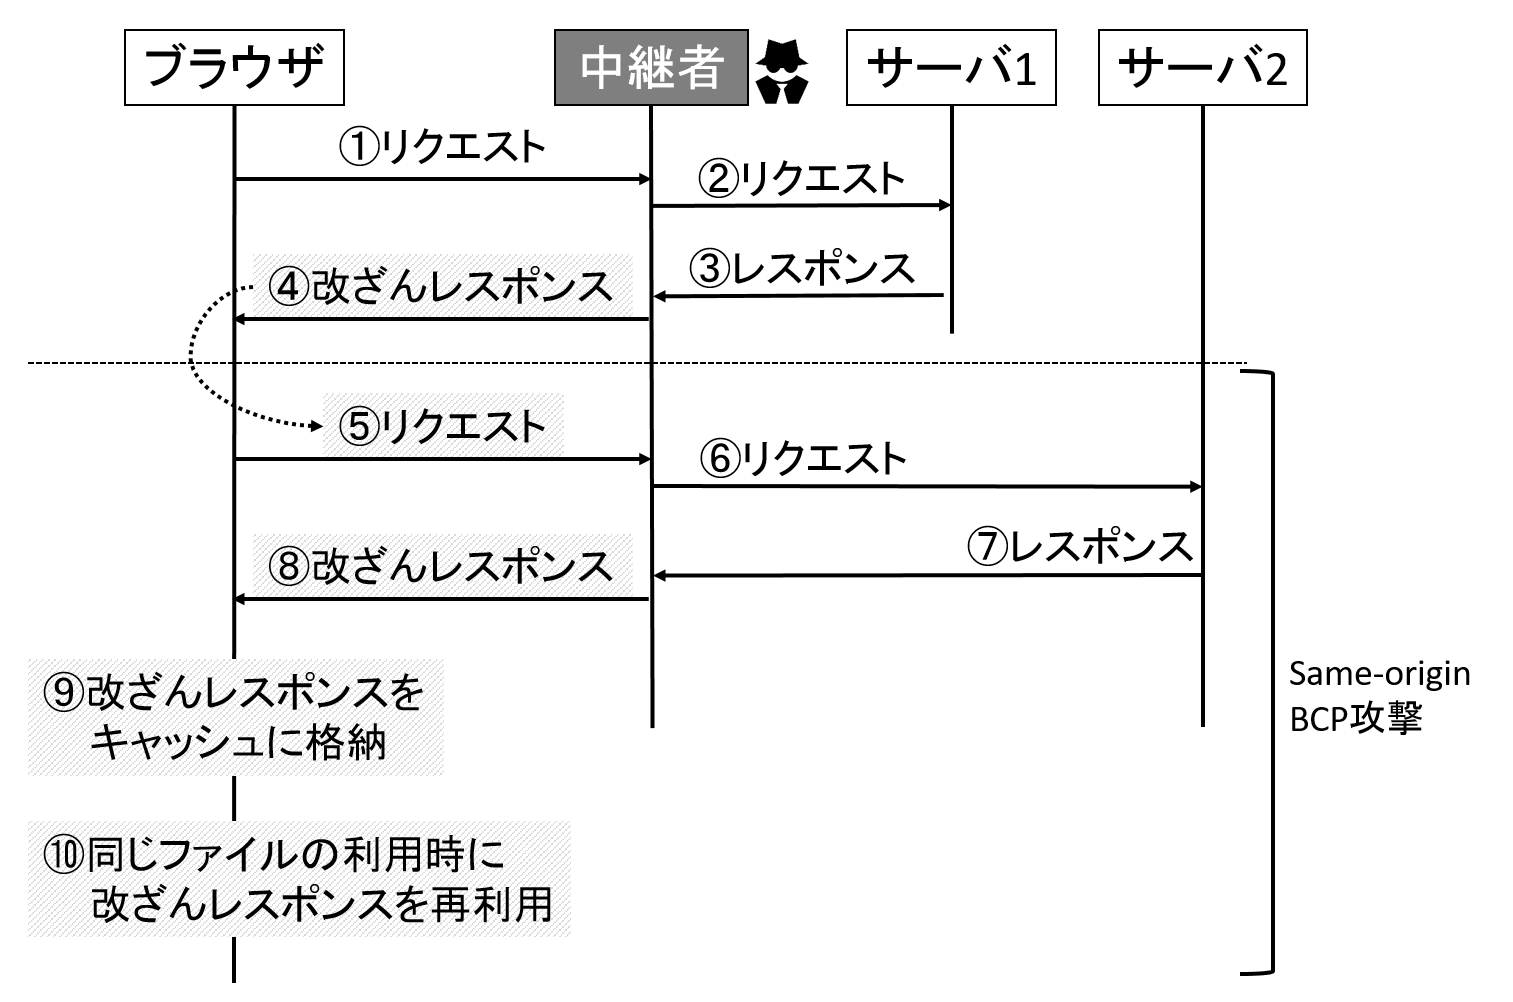
\includegraphics[width=450pt]{./fig/CrossBCP_flow.eps}
%\caption{Cross-origin Browser Cache Poisoning Attackの攻撃フロー}
%\label{fig:CrossBCP_flow}
%\end{figure}

提案モデルによるCross-origin BCP攻撃の表現を確認するため、実行結果から図\ref{fig:CrossBCP_flow}を含む結果を抽出する。
結果として、図\ref{fig:CrossBCP_flow}に存在する五つの通信を表現された状態を出力した。
このことから、提案モデルがCross-origin BCP攻撃を表現できることを確認した。
また、スペースの都合上、実行コードは巻末付録Code\ref{code:Cross_origin_BCP}に記載する。

\subsection{Web Cache Deception Attack}
本節では、提案モデルでWeb Cache Deception Attack\cite{WCD}(以下、WCD攻撃とする)が表現可能であるかを確認する。

WCD攻撃は攻撃対象となるサーバと中継者、二つのブラウザ間で成り立つ攻撃である。
攻撃者はこれらのうち一つのブラウザを所有し、本来、攻撃者がサーバから得ることのできないファイルを取得することが目的である。

WCD攻撃は図\ref{fig:WCD_flow}に示す攻撃フローで実現される。
まず、攻撃者にアクセス権の無いファイルに対して、正当なユーザに中継者を経由してアクセスさせる。
この際に、その「3.レスポンス」が中継者のキャッシュに格納された場合、攻撃者はその中継者を含む経路でそのファイルに対する「5.リクエスト」を送信することで、中継者のキャッシュによる「6.格納レスポンスの再利用」が発生しそのファイルを取得できる。

%\begin{figure}[htb]
%\centering
%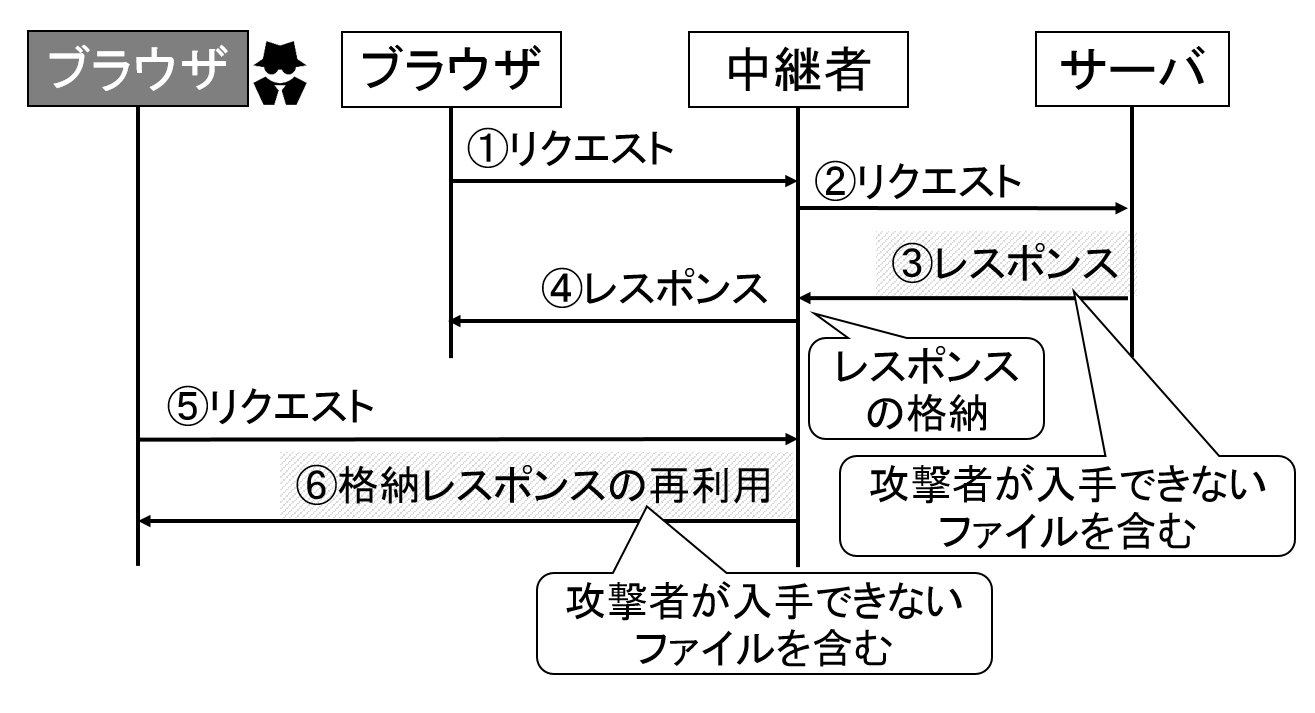
\includegraphics[width=450pt]{./fig/WCD_flow.eps}
%\caption{Web Cache Deception Attackの攻撃フロー}
%\label{fig:WCD_flow}
%\end{figure}

提案モデルによるWCD攻撃の表現を確認するため、実行結果から図\ref{fig:WCD_flow}のフローを含む結果を抽出する。
抽出にはCode\ref{code:WCD}を用い、その実行結果として図\ref{fig:WCD_flow}に示す攻撃フローを含む結果が出力された。
スペースの都合上、これを一部簡略化し図\ref{fig:WCD_alloy}に示す。
図\ref{fig:WCD_alloy}において、図\ref{fig:WCD_flow}の「1.リクエスト」と「2.リクエスト」の通信はStateTransaction0,1でそれぞれ表されている。
ここで、Response1のボディにはTokenが付与されており、これが攻撃者がアクセス権を持たないファイルを示している。
このResponse1は、その発生時刻Time2で中継者のキャッシュに保存され、攻撃者による通信StateTransaction2において再利用されている。
従って、この出力結果は攻撃者が本来権限を持たないファイルを中継者のキャッシュによる再利用を用いて取得していることを表している。
以上のことから、WCD攻撃を含む出力結果が得られているため、提案モデルがWCD攻撃を表現できることを確認した。

\begin{lstlisting}[caption=WCD攻撃の表現, label=code:WCD]
run Web_Cache_Deception{
	#HTTPRequest = 3
	#HTTPResponse = 2
	#CacheReuse = 1

	#HTTPClient = 2
	#HTTPServer = 1
	#HTTPProxy = 1
	#Cache = 1

	#Principal = 4
	#Alice = 3

	all c:Cache | c in HTTPProxy.cache

	all p:Principal |
		one c:HTTPConformist |
			c in p.(servers + httpClients)
	all i:HTTPProxy | i in Alice.servers
	all s:HTTPServer | s in Alice.servers

	one tr1,tr2,tr3:HTTPTransaction |{
		tr1.request.from in Alice.httpClients
		tr1.request.to in HTTPProxy

		tr2.request.from in HTTPProxy
		tr2.request.to in HTTPServer

		(tr3.request.from !in Alice.httpClients and tr3.request.from in HTTPClient)
		tr3.request.to in HTTPProxy

		one tr3.re_res
	}
} for 6
\end{lstlisting}

%\begin{figure}[htb]
%\centering
%\includegraphics[width=450pt]{./fig/WCD_alloy.eps}
%\caption{WCD攻撃のフローを含む状態の一例}
%\label{fig:WCD_alloy}
%\end{figure}

\end{document}
